
In this chapter, we evaluate our quantification model and inference algorithms on simulated datasets with constant expected degradation rates and real direct RNA-seq datasets with sequencing spike-ins. 

\section{Existing methods}

We benchmark our model against existing methods for transcript quantification from long-read RNA-seq:
\begin{itemize}
    \item Bambu
    \item Flair
    \item Nanocount
\end{itemize}

\section{Simulated data}

To evaluate our model's ability to correct for degradation bias, we simulate five datasets for a range of degradation rates $\mathbb{E}[d]\in\{0.05,0.1,0.2,0.4,0.5\}$. In addition, we simulate reads for artificial novel isoforms that are modified by dropping exons from the 5' end of selected reference isoforms, termed \textit{subset} isoforms. This increases the proportion of multi-mapping reads and makes correcting for degradation bias crucial for accurate transcript quantification. See Appendices \ref{ap:gen-novl-iso} and \ref{ap:sim-deg-reads} for more details on novel isoform and degraded read simulation. 

\subsection{Empirical results}

\begin{figure}[H]
    \centering
    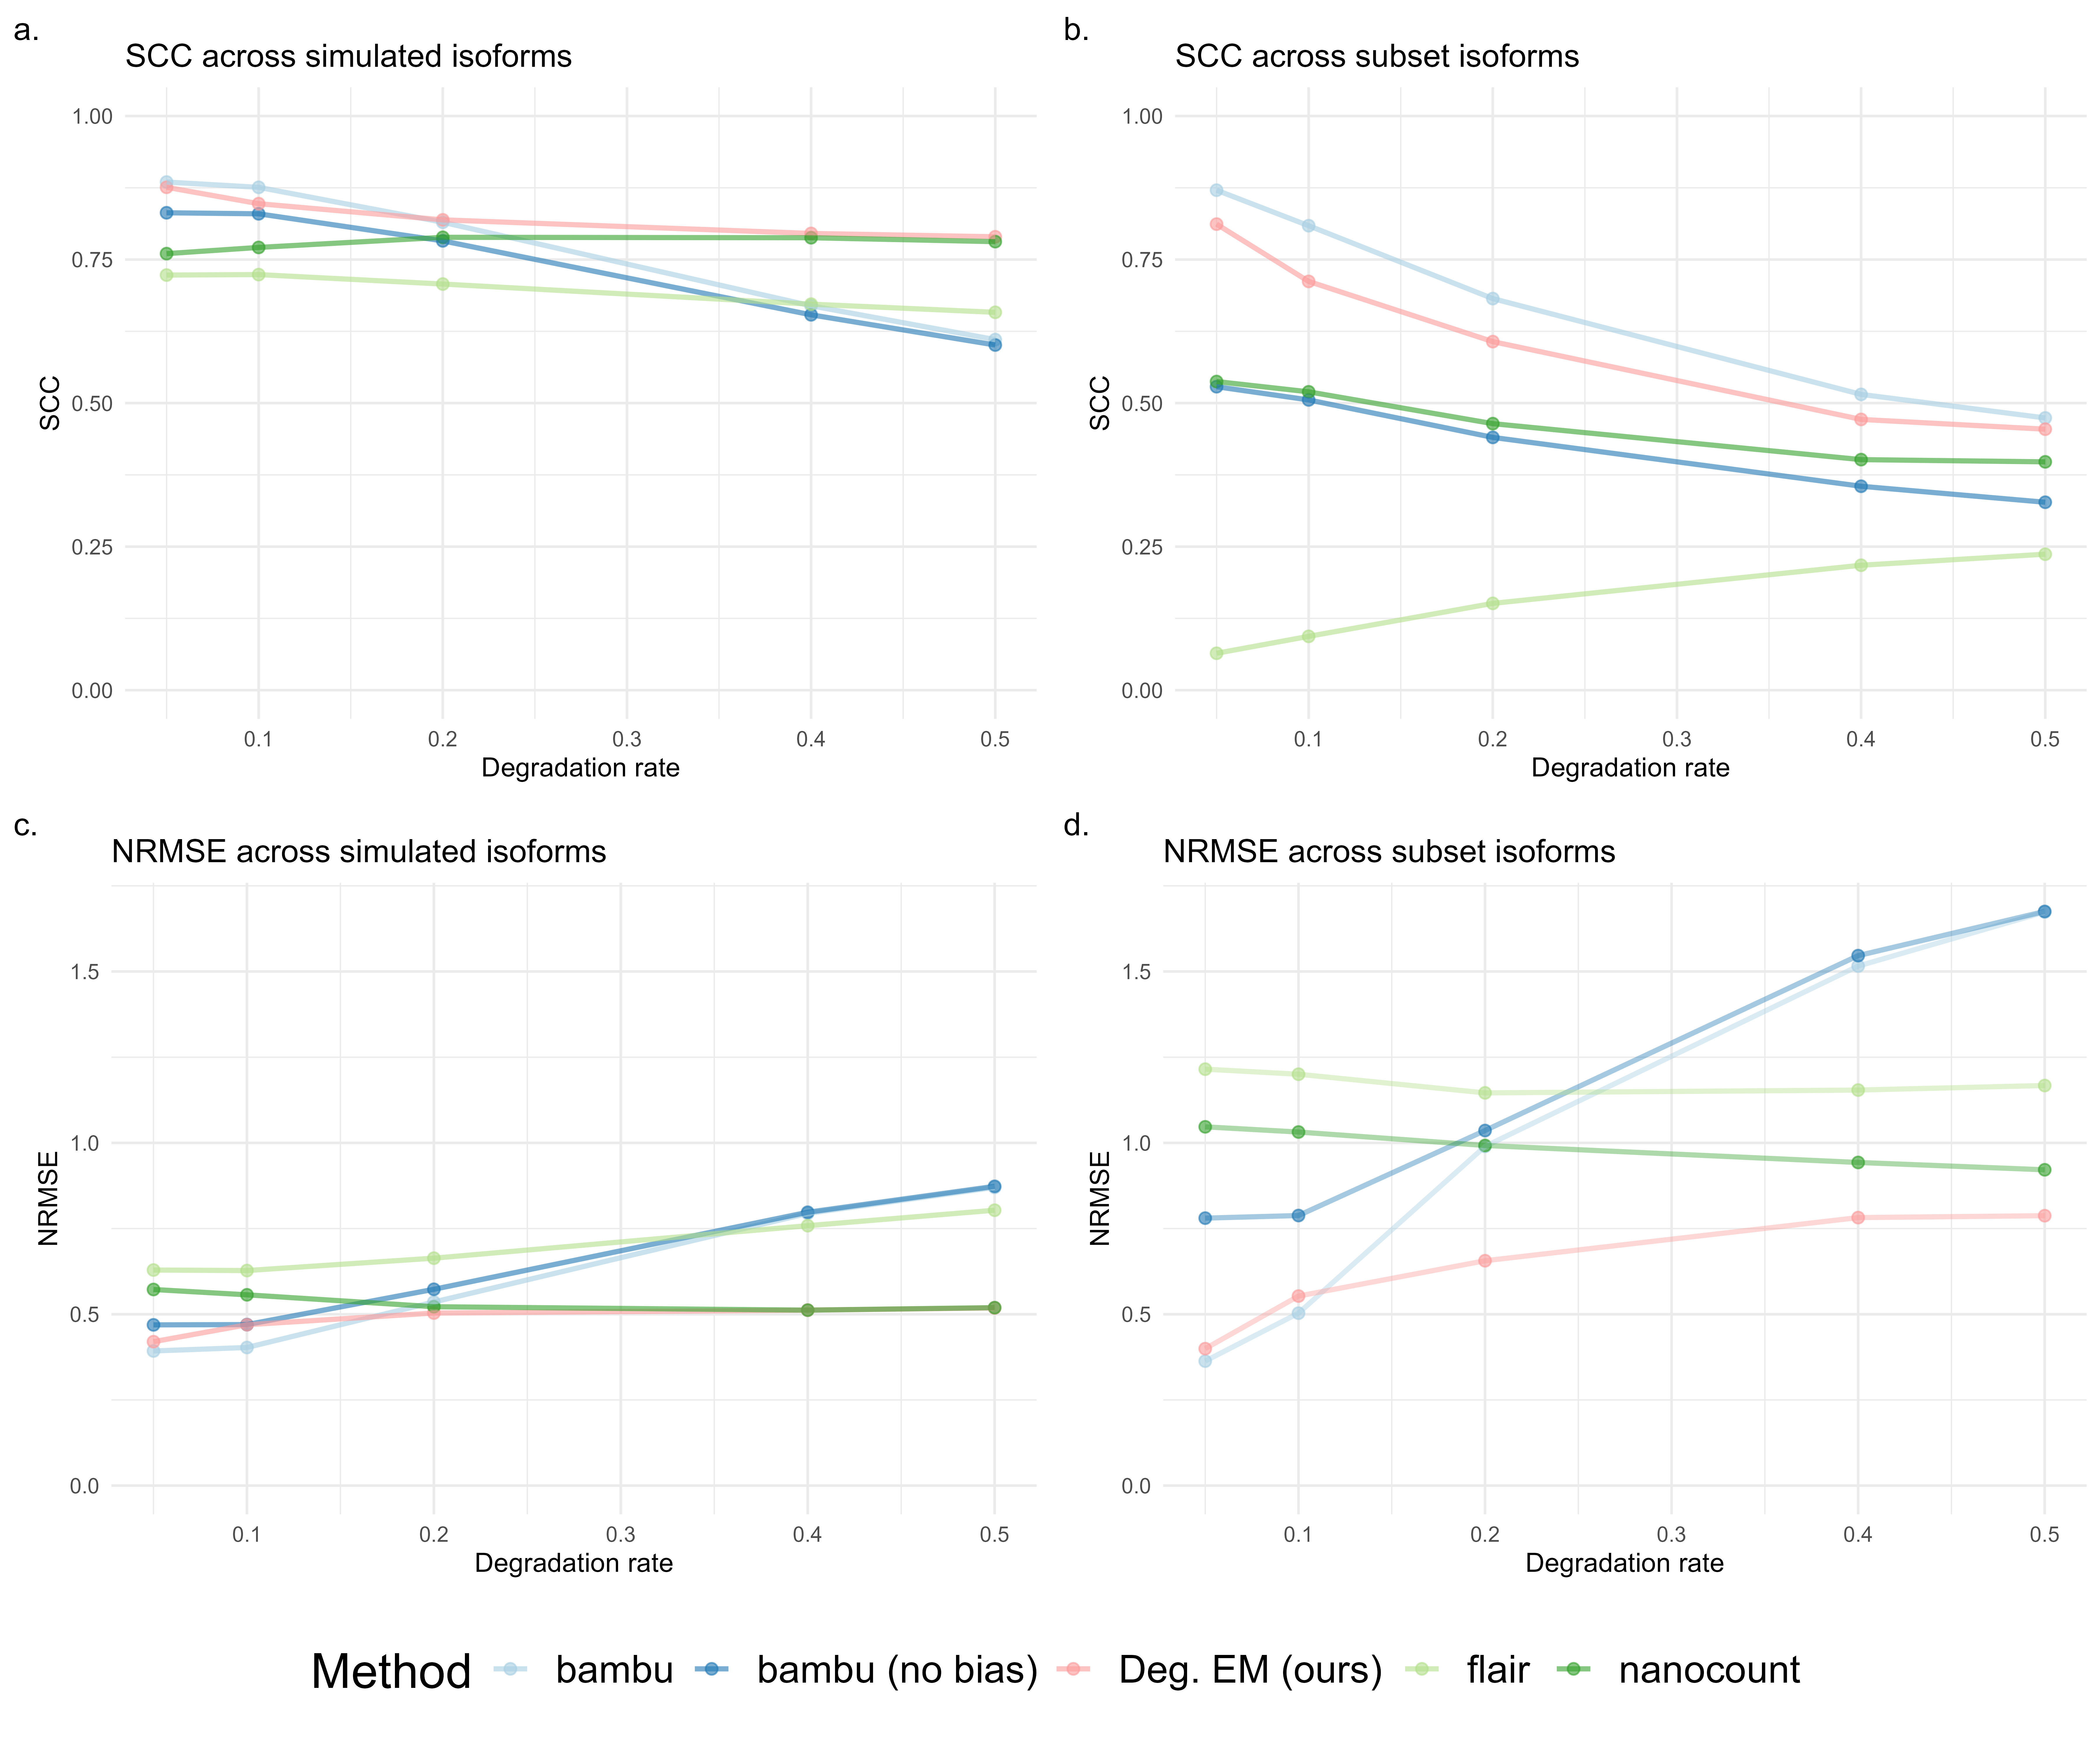
\includegraphics[width=\textwidth]{figures/sec-3-scc-nrmse.png}
    \caption[Empirical results for SCC and NRMSE on simulated datasets]{Spearman correlation coefficient (SCC) and normalized root-mean-squared error (NRMSE) on simulated datasets with different degradation rates $\mathbb{E}[d]=\{0.05,0.1,0.2,0.4,0.5\}$. \textbf{a.} SCC across all simulated isoforms. \textbf{b.} SCC across subset isoforms. \textbf{c.} NRMSE across all simulated isoforms. \textbf{d.} NRMSE across all subset isoforms.}
    \label{fig:sec-3-scc-nrmse}
\end{figure}

\begin{figure}[H]
    \centering
    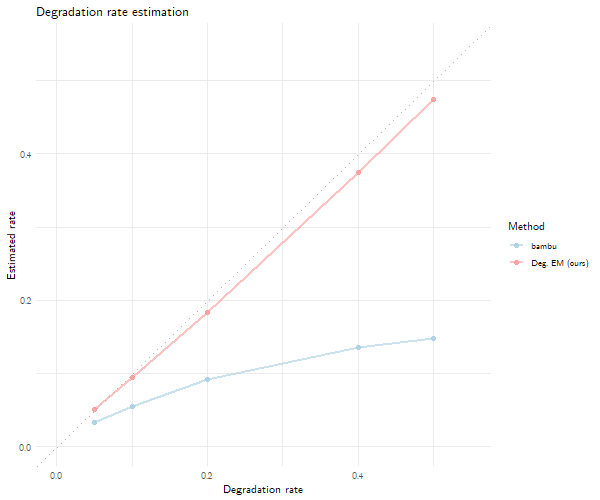
\includegraphics[width=0.7\textwidth]{figures/sec-3-deg-est.png}
    \caption[Empirical results for degradation rate estimation on simulated datasets]{Comparison of the degradation rates estimated by bambu and our model on simulated datasets with different degradation rates $\mathbb{E}[d]=\{0.05,0.1,0.2,0.4,0.5\}$.}
    \label{fig:sec-3-deg-est}
\end{figure}


\begin{table}[htbp]
  \centering
    \begin{tabular}{|l|P{2cm}|P{2cm}|P{2cm}|P{2cm}|}
\cline{2-5}    \multicolumn{1}{r|}{} & \multicolumn{2}{c|}{All isoforms} & \multicolumn{2}{c|}{Subset isoforms} \bigstrut\\
    \hline
    Method & SCC   & NRMSE & SCC   & NRMSE \bigstrut\\
    \hline
    bambu & 0.771 & 0.599 & 0.671 & 1.009 \bigstrut\\
    \hline
    bambu (no bias) & 0.74  & 0.636 & 0.432 & 1.165 \bigstrut\\
    \hline
    Deg. EM & 0.826 & 0.485 & 0.612 & 0.635 \bigstrut\\
    \hline
    Deg. EM (emp.) & \textbf{0.874} & \textbf{0.393} & \textbf{0.811} & \textbf{0.43} \bigstrut\\
    \hline
    flair & 0.697 & 0.696 & 0.153 & 1.176 \bigstrut\\
    \hline
    nanocount & 0.778 & 0.536 & 0.466 & 0.987 \bigstrut\\
    \hline
    \end{tabular}%
    \caption[Empirical results for mean SCC and NRMSE on simulated datasets]{Mean spearman correlation coefficient (SCC) and normalized root-mean-squared error (NRMSE) across simulated datasets with different degradation rates $\mathbb{E}[d]=\{0.05,0.1,0.2,0.4,0.5\}$.}
  \label{tab:addlabel}%

\end{table}%

\section{Real data}

\subsection{Empirical results}